% Created 2021-01-24 Sun 22:50
% Intended LaTeX compiler: pdflatex
\documentclass[11pt]{article}
\usepackage[utf8]{inputenc}
\usepackage[T1]{fontenc}
\usepackage{graphicx}
\usepackage{grffile}
\usepackage{longtable}
\usepackage{wrapfig}
\usepackage{rotating}
\usepackage[normalem]{ulem}
\usepackage{amsmath}
\usepackage{textcomp}
\usepackage{amssymb}
\usepackage{capt-of}
\usepackage{hyperref}
\usepackage{minted}
\hypersetup{colorlinks=true, linkcolor=black, filecolor=red, urlcolor=blue}
\usepackage[turkish]{babel}
\author{Eren Hatırnaz}
\date{17 Kasım 2019}
\title{Yazılım Gündemi - 18\\\medskip
\large 11-17 Kasım 2019}
\hypersetup{
 pdfauthor={Eren Hatırnaz},
 pdftitle={Yazılım Gündemi - 18},
 pdfkeywords={},
 pdfsubject={},
 pdfcreator={Emacs 27.1 (Org mode 9.3)},
 pdflang={Turkish}}
\begin{document}

\maketitle
\tableofcontents \clearpage\shorthandoff{=}

\begin{center}
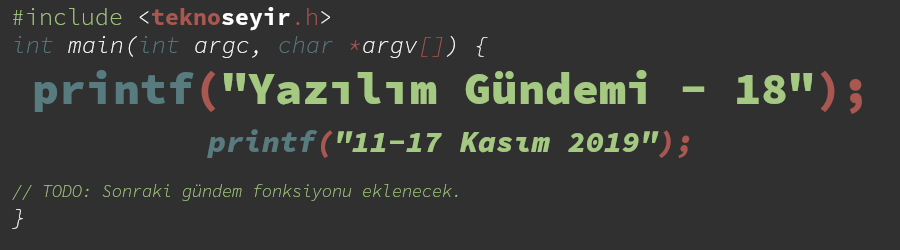
\includegraphics[width=.9\linewidth]{gorseller/yazilim-gundemi-banner.png}
\end{center}

\begin{center}
\href{../17/yazilim-gundemi-17.pdf}{< Önceki Gündem} | \textbf{11-17 Kasım 2019} | \href{../19/yazilim-gundemi-19.pdf}{Sonraki Gündem >}

\href{https://teknoseyir.com/blog/yazilim-gundemi-18-11-17-kasim-2019}{TeknoSeyir'de Oku}
\end{center}

\section{\href{https://githubuniverse.com/}{GitHub Universe 2019} etkinliği \href{https://github.blog/2019-11-13-universe-day-one/}{gerçekleşti}}
\label{sec:org656229e}
GitHub'ın her yıl geleneksel olarak düzenlediği Universe etkinliği bu sene de,
bu hafta içerisinde gerçekleşti. Etkinlik ABD'deki Kaliforniya eyaletinde
gerçekleşti fakat aynı zamanda canlı yayın ile de tüm dünyaya yayınlandı. Ben
etkinliği izleyemedim ama etkinlikle duyurdukları her şeyi toparladıkları blog
yazısını inceledim ve sizlere birkaç tane geliştmeyi aktarmaya çalışacağım.
Öyleyse başlayalım:

\subsection{GitHub iOS uygulamasının Beta programı duyuruldu}
\label{sec:org6a2716d}
Mobilden GitHub'a erişebilmek bazen benim de ihtiyaç duyduğum bir şeydi. Şu an
zaten mobil tarayıcıdan GitHub'a girdiğinizde ona göre bir arayüz geliyor
fakat yine pek kullanışlı değil. iOS uygulama mağazasında bazı üçüncü parti
uygulamalar olsa da ben pek güvenemedim. Sonuçta tüm depolarımıza erişim izni
veriyoruz. GitHub da bu alanda bir eksiklik hissetmiş olacak ki bu etkinlikle
iOS uygulamasının beta sürecinin başladığını \href{https://twitter.com/github/status/1194675248047616000}{duyurdu}. Android için ise yakında
başlayacağını belirttiler. Duyar duymaz ben de hemen Beta için kayıt yaptım ve
3-4 gündür kullanıyorum. Siz de iOS uygulamanın beta programına kaydolmak için
\href{https://github.com/mobile/beta?platforms=ios}{buraya}; Android uygulamanın bekleme listesine kaydolmak için \href{https://github.com/mobile/beta?platforms=android}{buraya}
tıklayabilirsiniz.

\begin{center}
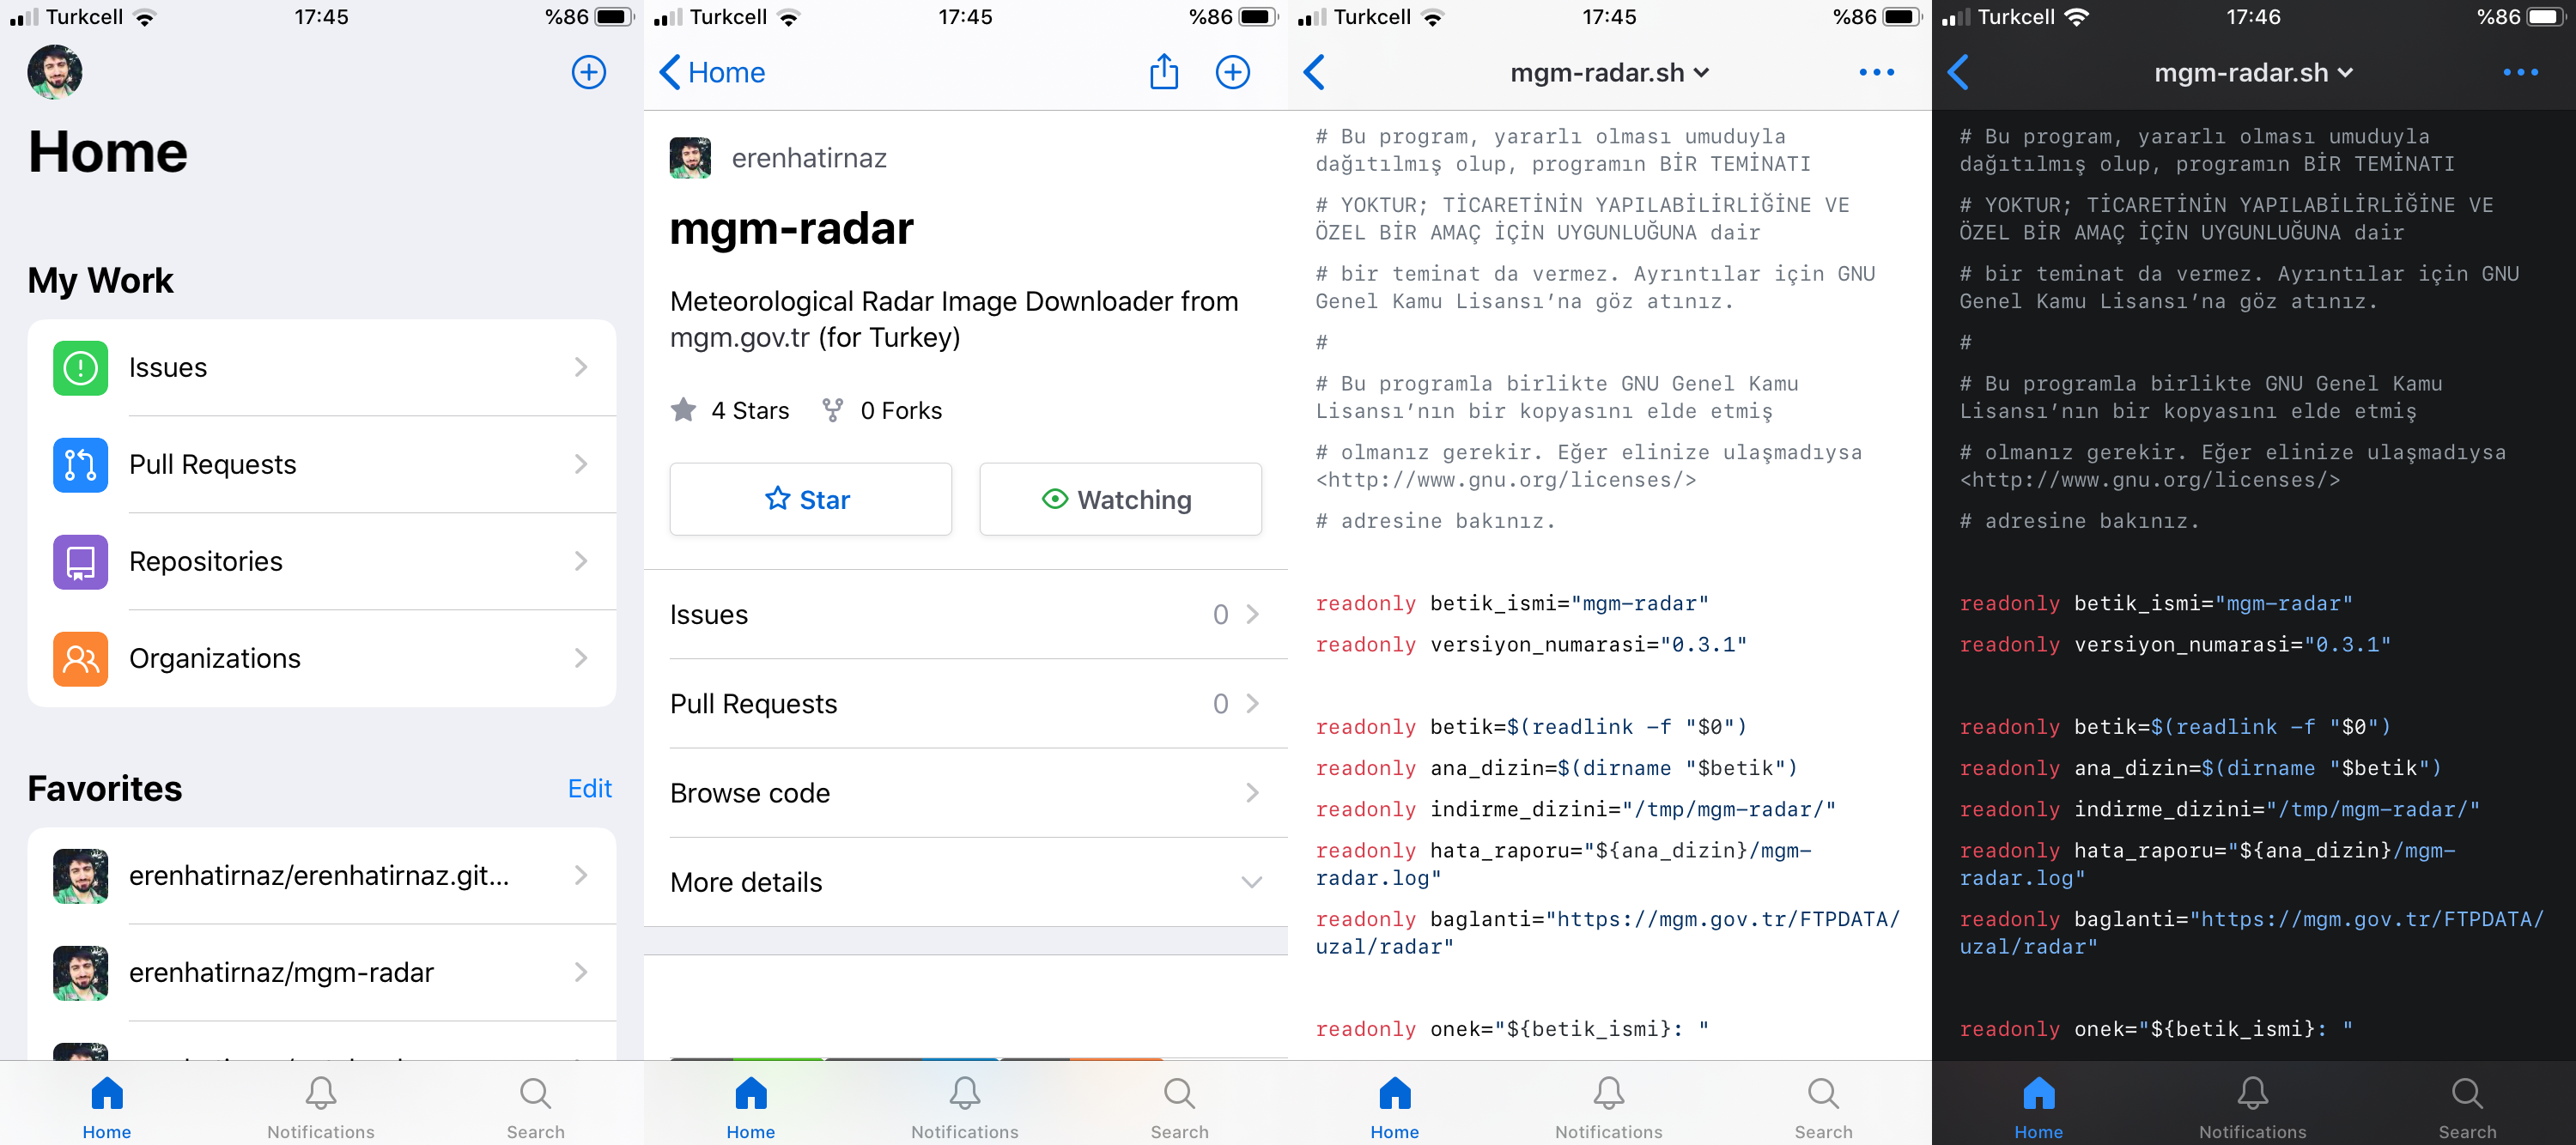
\includegraphics[width=.9\linewidth]{gorseller/github-mobile-ios.png}
\end{center}

Kullandığım kadarıyla gayet güzel bir uygulama olmuş fakat şu an için
eksikleri ve hataları mevcut. Örneğin hangi branch'da olduğumu göremiyorum ya
da branch'lar arasında geçiş yapamıyorum (bence olması gereken bir özellik).
README.md dosyalarındaki görsellerde de gözükmeme sorunu mevcut. Ayrıca gece
moduna teması da mevcut. İşin ilginci GitHub web'de henüz gece modu teması
yok. Umarım web sürümüne de gelir. Geceleri GitHub'ı açtığımda far görmüş
tavşan gibi kalmak istemiyorum. Gerekli geri bildirimleri mail olarak
gönderdim. Gerekli geliştirmeler devam edecektir.
\subsection{GitHub Arşiv Programı duyuruldu}
\label{sec:org5252ac7}
GitHub herkese açık depolarımızı 1000 yıl boyunca saklamak için hazırlanıyor.
Birkaç ülkenin meyve ve sebze tohumları için yaptığı çalışmanın aynısını
GitHub da kodlarımız için yapmak için kollarını sıvadı. Bu etkinlikte
duyurulan bu programın amacı ise gelecek nesillere şimdiki zamanın programlama
kültürü ile ilgili materyaller bırakmak. Bu sayede geleceğin tarihçileri ya da
"dijital arkeolojist"leri bu depoları inceleyerek programlama kültürümüz ya da
topluluklarımız ile ilgili bilgiler edinebilecekler ya da bambaşka amaçlar
için kullanabilirler -kim bilir.

Elbette GitHub bu işi tek başına yapmıyor. Partnerlerin hepsini tek tek yazmak
yerine programdaki rollerini açıklayarak ilerleyelim.

\begin{itemize}
\item GitHub: Zaten tüm verileri sağlayan şirketin kendisi. GitHub neredeyse
anlık olarak tüm depolara ait verileri API sistemi üzerinden erişilebilir
şekilde diğer partnerler ile paylaşacak.
\item GHTorrent: GitHub'ın tüm herkese açık verilerini takip edecek ve bunları
günlük ya da aylık formatlarda erişilebilecek şekilde saklayacak.
\item GH Archive: GHTorrent'e ek olarak bu hizmet aynı zamanda BigQuery
kullanarak sorgulama özelliği de sunacak. Bu hizmetten de saatlik, günlük
ya da aylık şekilde indirmeler yapabileceğiz.
\item Internet Archive: Zaten birçok farklı web sitenin eski hallerini saklayan
bu hizmet aynı şeyi GitHub depolarının sayfaları için de yapacak ve
bunlara git veya https üzerinden erişilebilecek.
\item Software Heritage Foundation: Aylık olarak GitHub'ı tarayacak ve herkese
açık verileri kendi arşivine alacak.
\item Bodleian Kütüphanesi: Oxford Üniversite'ne bağlı bu kütüphane GitHub'daki
en çok yıldız alan ve en çok proje tarafından kullanılan projeleri kendi
depolarında (repo değil, fiziksel depo) film makaralarında saklayacak.
\item Arctic World Archive: 2 Şubat 2020 tarihinde alınacak tüm aktif herkese
açık depoların görüntüleri (snapshot) yine film makaralarında, kuzey
kutbuna çok yakın bir yerde uzun ömürlü olacak şekilde depolanacak.
\item Microsoft Project Silica: Her beş yılda bir olacak şekilde Microsoft
Resarch takımı aktif ve herkese açık tüm depoları 10.000 yıl
saklayabilecek quartz cam plakalara femtosecond lazer kullarak yazacak.
\end{itemize}

Gördüğünüz gibi bayağı büyük bir organizasyon şeklinde işleyecek bu program.
Diğer detaylı ayrıntılar için GitHub'ın hazırladığı \href{https://archiveprogram.github.com/}{bu web sayfasını} ziyaret
edebilirsiniz. Açıkcası her ne kadar gelecekler kodlarımızın ne amaçla
kullanılacağını bilmesek de program benim hoşuma gitti. Hatta güzel birkaç
bilim-kurgu senaryosu da aklıma geldi konuyla ilgili.

Bu konuyla ilgili siz ne düşünüyorsunuz? Sizce gelecekte kodlarımız hangi
amaçlar için kullanılabilir? Yorumlar bölümünde beyin fırtınası yapalım.

Etkinlikle duyurulan diğer birkaç gelişme ise şu şekilde:
\begin{itemize}
\item \href{https://github.blog/2019-11-13-universe-day-one/\#github-actions}{GitHub Actions} ve \href{https://github.blog/2019-11-13-universe-day-one/\#github-packages}{GitHub Packages} beta programından çıktılar,
\item Bildirimlerde \href{https://github.blog/2019-11-13-universe-day-one/\#notifications}{iyileştirmeler},
\item Bir fonksiyonun nerede tanımlandığını ya da nerelerde kullanıldığını
\href{https://github.blog/2019-11-13-universe-day-one/\#navigation}{gösterme},
\item Kodlar içerisinde özel \href{https://github.blog/2019-11-13-universe-day-one/\#search}{aramalar yapabilme},
\item GitHub Güvenlik Labaratuvarı \href{https://github.blog/2019-11-14-announcing-github-security-lab-securing-the-worlds-code-together/}{tanıtıldı},
\item GitHub Enterprise Server 2.19 sürümü \href{https://github.blog/2019-11-13-universe-day-one/\#server}{duyuruldu},
\end{itemize}
Ayrıca bu hafta içerisinde GitHub'ın Kullanım Sözleşmesi ve Gizlilik Anlaşması
da \href{https://github.blog/2019-11-15-updates-to-our-terms-of-service-and-privacy-statement/}{güncellendi}.
\section{Mozilla, Bytecode Birliğini \href{https://hacks.mozilla.org/2019/11/announcing-the-bytecode-alliance/}{tanıttı}}
\label{sec:org4d8b700}
\begin{center}
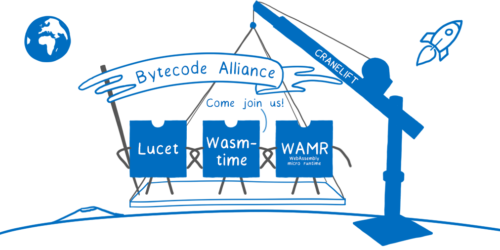
\includegraphics[height=3cm]{gorseller/mozilla-bytecode-alliance.png}
\end{center}

Tek amacı olmasa da en büyük amaçlarından biri olan JavaScript'e alternatif
olması için geliştirilen WebAssembly programlama diline en çok katkı
yapanlardan birisi olan Mozilla, topluluk için çalışmaya devam ediyor. Elbette
birliği tek başına kurmadı. Şu an için birliğin içerisinde Fastly, Intel ve Red
Hat firmaları var fakat daha çok firmanın da katılmasını bekliyorlar.

Günümüzde yazılım geliştirmenin evrildiği hal itibariyle üçüncü parti
kütüphaneler olmadan bir yazılım çözümü üretmek neredeyse imkansız hale geldi.
Elbette üçüncü parti kütüphaneler ya da araçlar kullanmanın kötü bir yanı yok,
aksine açık kaynak topluluğu için çok faydalı da oluyor fakat bu sürecin
sağlıklı olmayan bazı parçaları mevcut. Şöyle ki, kullanıcı bir uygulamayı
sistemine kurduğunda ya da tarayıcısı üzerinden çalıştırdığında beraberinde o
uygulamanın bağımlı olduğu tüm kütüphaneleri de sistemine indiriyor ve
çalıştırıyor. Fakat uygulamayı çalıştırarak ona güvendiğini belirten bu
kullanıcının, uygulamanın beraberinde getirdiği kütüphanelere ya da araçlara
güvenmesi için bir neden yok (aslında geliştirici olarak bizim de güvenmemiz
için bir neden yok). Bunun somut örneklerini önceki yazılım gündemi yazılarında
çokça aktarmıştım (zararlı kod içeren 3.parti kütüphaneden, kötü amaçlı
kişilerin ellerine geçmiş kütüphanelere kadar örnekler mevcut). İşte bu
birliğin amacı da WebAssembly ekosistemi için tam olarak bu güven ortamını
yaratmak.

Konu hakkında siz ne düşünüyorsunuz? Sizce de artık üçüncü parti kütüphane ve
araçlara bakış açımızı değiştirme zamanı geldi mi? Sizin üçüncü parti kütüphane
seçerken dikkat ettiğiniz şeyler neler? Yorumlar kısmında konuşalım.
\section{OpenJDK kod tabanını GitHub'a \href{https://www.infoworld.com/article/3453397/openjdk-repo-migration-to-github-gains-steam.html}{taşımayı tartışıyor}}
\label{sec:orgbbc601a}
Java'nın açık kaynak sürümü olan OpenJDK, bu sıralar çeşitli önerileri
tartışmakla meşgul. Bunlardan bu sıralar gündemde olanları ise şu şekilde:
\begin{itemize}
\item \href{https://openjdk.java.net/jeps/296}{JEP 296: Consolidate The JDK Forest into a Single Repository}
\item \href{https://openjdk.java.net/jeps/357}{JEP 357: Migrate from  Mercurial to Git}
\item \href{https://openjdk.java.net/jeps/369}{JEP 369: Migrate to GitHub}
\end{itemize}
Bunlardan ilki şu sıralar birçok firmanın da uygulamaya başladığı yeni bir moda
olan mono-repo sistemine geçmeyi öneriyor. Yani tüm kod tabanının büyük tek bir
depoda tutulduğu yapı. İkincisi ise Git'den daha önce de var olan bir versiyon
kontrol sistemi olan Mercurial'den Git'e geçmeyi öneriyor ve sonuncusu ise
bugün konuşacağımız tüm kod tabanının GitHub'a taşınmasını öneriyor. Fakat
burada belirtmekte fayda var sadece kodların GitHub'a taşınması düşünülüyor;
issue tracker, wiki vb. yapılar yine olduğu yerde kalacaklar.

Öneri metini bayağı ayrıntılı bir şekilde hazırlanmış. Aynı metinde yer alan
"Hedefler" başlığındaki birkaç taşınma nedeni ise şu şekilde:
\begin{itemize}
\item Geliştiriciler katkı yapmak için OpenJDK'ya özel bazı araçları kurmak
zorunda kalmayacaklar,
\item Commit öncesi kontroller çalıştırabilme,
\item Mevcut e-posta tabanlı iş akışlarının benzerlerini desteklemesi,
\item GitHub'ın erişilebilirlik özelliklerinden faydalanabilme
\end{itemize}
gibi özellikler OpenJDK takımını cezbeliyor. İlgili önerilerin metinlerini
içeren sayfaları yukarıda maddeler hallinde bağlantı olarak ekledim. Daha
detaylı bilgi için oraları kontrol edebilirsiniz.
\section{Sourcehut, \href{https://sourcehut.org/blog/2019-11-15-sourcehut-1-year-alpha/\#expectations-for-2020}{2019 yılı özetini yayınladı}}
\label{sec:org6c19d9f}
Günümüzde artık bir versiyon kontrol sistemi olmadan geliştirme yapmak imkansız
olmasa bile çok zor. Çoğumuz da artık versiyon kontrol sistemi olarak Git'i
varsayılan olarak kullanmaya başladık. Hatta proje klasörünü oluşturduktan
sonraki ilk işimiz \texttt{git init} komutunu çalıştırmak oluyor. Bu lokal Git
depolarından ziyade çoğumuz artık kodlarımızı bir uzak Git sunucusunda da
tutmak istiyoruz. Bunların en popülerleri ise GitHub ve GitLab gibi büyük
oyuncular. Fakat ben bugün size pek gündemde olmayan, ilk yazılım gündemi
yazısını okumadıysanız muhtemelen ilk kez duyacağınız farklı bir uzak kod
sunucusundan, Sourcehut'dan bahsetmek istiyorum. Çünkü bu hafta 15 Kasım
tarihinde Alpha sürecine girmesinin birinci yılı şerefine bir blog yazısı
yayınlandı.

Sourcehut aslında sadece bir uzak kod sunucusu değil; günümüz uygulama
geliştirme süreçlerinde sürekli ihtiyaç duyduğumuz şu hizmetleri de olan komple
bir proje yönetim sistemi diyebiliriz:
\begin{itemize}
\item Kodlarınızı depolayabileceğiniz: \href{https://git.sr.ht/}{git.sr.ht},
\item Çeşitli testleri belirli aralıklarla çalıştırabileceğiniz Continuous
Integration sistemi: \href{https://builds.sr.ht/}{builds.sr.ht},
\item Yapılacaklar listesi ve hata bildirimi gibi şeyler için: \href{https://todo.sr.ht/}{todo.sr.ht},
\item Mail listesi için: \href{https://lists.sr.ht/}{lists.sr.ht},
\item Rehber ve Wiki sayfaları hazırlamak için: \href{https://man.sr.ht/}{man.sr.ht}
\end{itemize}
ve tüm bu çözümleri arayüzü gibi sade olarak sunmaya çalışan bir site. Elbette
tüm bu sistemler özgür yazılım lisanslarıyla geliştiriliyor.

Bir yıl içerisinde Sourcehut'daki gelişmelerin bir kısmı ise şu şekilde:
\begin{itemize}
\item Code Annotations özelliği (bkz: \href{../01/yazilim-gundemi-01.pdf}{Yazılım Gündemi - 1}),
\item builds.sr.ht'de çalışan testlerin olduğu sanal makineye debug yapmak için
ssh ile bağlanabilme,
\item todo.sr.ht üzerindeki ticket sistemi olgunlaştırılmış,
\item ilk çalışan işe alınmış
\end{itemize}

Diğer gelişmeler ve 2020 yılından beklentiler için mutlaka konu başlığına
eklediğim blog yazısını inceleyin. Ben şahsen bu projeyi çok önemsiyorum ve
ileride imkanım olduğunda maddi olarak da destek olmaya çalışacağım.
\newpage
\section{Yaklaşan Etkinlikler}
\label{sec:orgfb4002a}
\begin{longtable}{|p{8cm}|l|l|}
\hline
Etkinlik İsmi & Yeri & Tarihi\\
\hline
\endfirsthead
\multicolumn{3}{l}{Önceki sayfadan devam ediyor} \\
\hline

Etkinlik İsmi & Yeri & Tarihi \\

\hline
\endhead
\hline\multicolumn{3}{r}{Devamı sonraki sayfada} \\
\endfoot
\endlastfoot
\hline
\href{https://www.eventbrite.com/e/open-source-yazlm-gelistirme-akaunting-kurucu-ortag-denis-dulici-tickets-79951076823}{Open Source Yazılım Geliştirme} & İstanbul & 20 Kasım 18:30\\
\href{https://kommunity.com/software-craftsmanship-turkey/events/tum-interneti-nasil-cacheleriz-olasiliksal-veri-yapilarina-yolculuk}{Tüm İnterneti Nasıl Cache'leriz? Olasılıksal Veri Yapılarına Yolculuk} & İstanbul & 20 Kasım 19:00\\
\href{https://kommunity.com/atolye15/events/how-to-get-better-at-writing-css}{How to Get Better at Writing CSS} & İzmir & 20 Kasım 19:00\\
\href{https://www.eventbrite.com/e/kworks-inovatif-endustriyel-iot-uygulamalar-paneli-tickets-80823638679}{KWORKS İnovatif Endüstriyel IoT Uygulamaları Paneli} & İstanbul & 21 Kasım 18:00\\
\href{https://www.eventbrite.com/e/web-uygulama-guvenligi-ve-bug-bounty-hacknightsorg-tickets-78021938719}{Web Uygulama Güvenliği ve Bug Bounty} & Ankara & 21 Kasım 19:00\\
\href{https://kommunity.com/sap-community-turkey/events/sap-inside-track-istanbul-2019-part-ii}{SAP Inside Track Istanbul 2019 Part II} & İstanbul & 23 Kasım 09:00\\
\href{https://www.eventbrite.com/e/gdg-devfest-izmir-19-tickets-75047965485}{GDG DevFest İzmir '19} & İzmir & 23 Kasım 09:00\\
\href{https://kommunity.com/istanbulphp/events/kubernetes-native-uygulama-gelistirme}{"Kubernetes Native" Uygulama Geliştirme} & İstanbul & 23 Kasım 13:00\\
\href{https://devfest.istanbul/}{GDG DevFest İstanbul '19} & İstanbul & 24 Kasım 09:00\\
\href{https://www.eventbrite.com/e/gelisen-teknoloji-gunleri19-tickets-82196167951}{Gelişen Teknoloji Günleri'19} & İstanbul & 26 Kasım 09:30\\
\href{https://kommunity.com/digitalzone-meetups-aylik-seo-kafe-toplantilari/events/digitalzone-meetups-26-kasim-bulusmasi}{Digitalzone Meetups: 26 Kasım Buluşması} & İstanbul & 26 Kasım 19:00\\
\href{https://www.eventbrite.com/e/sosyal-muhendislik-saldrlar-ve-korunma-yontemleri-hacknightsorg-tickets-77644170805}{Sosyal Mühendislik Saldırıları ve Korunma Yöntemleri} & İstanbul & 27 Kasım 19:00\\
\href{https://www.eventbrite.com/e/yapay-zekada-bias-calstay-registration-79316901989}{Yapay Zekada Bias Çalıştayı} & İstanbul & 30 Kasım 09:30\\
\href{https://www.acikhack.com/}{Açık Hack} & Gebze/Kocaeli & 30 Kasım 12:00\\
\hline
\end{longtable}
\section{Diğer Haberler}
\label{sec:orged48157}
\begin{itemize}
\item Go programlama dilinin artık paket arama vb. işler için \href{https://blog.golang.org/go.dev}{yeni bir sitesi var}:
\href{https://go.dev/}{go.dev}
\item Mirantis firması, Docker'ın Enterprise kısmını \href{https://techcrunch.com/2019/11/13/mirantis-acquires-docker-enterprise/}{satın aldı}.
\item AWS yeni hizmetini \href{https://aws.amazon.com/tr/blogs/aws/aws-data-exchange-find-subscribe-to-and-use-data-products/}{duyurdu}: \href{https://aws.amazon.com/data-exchange/}{AWS Data Exchange}.
\item PHP 7.4.0 RC6 sürümü \href{https://news-web.php.net/php.internals/107792}{yayınlandı}.
\item GitHub'ın Göçmenlik ve Gümrük Muhafaza kurumu ile yaptığı iş anlaşmasının
\href{https://techcrunch.com/2019/11/13/github-faces-more-resignations-in-light-of-ice-contract/}{etkileri devam ediyor}.
\item \href{https://www.redhat.com/en/technologies/cloud-computing/quay}{RedHat Quay} isimli projenin açık kaynak hali \href{https://www.projectquay.io/}{Project Quay} ismiyle \href{https://www.redhat.com/en/blog/red-hat-introduces-open-source-project-quay-container-registry}{duyuruldu}.
\item "Redux Starter Kit" artık hayatına "\href{https://redux-toolkit.js.org/}{Redux Toolkit}" olarak \href{https://github.com/reduxjs/redux-toolkit/releases/tag/v1.0.4}{devam edecek}.
\item Android geliştirme ile ilgili sürüm güncelleştirmeleri:
\begin{itemize}
\item \href{https://androidstudio.googleblog.com/2019/11/emulator-2929-and-amd-hypervisor-12-to.html}{Android Emulator 20.2.9 ve AMD Hypervisor 1.2 Canary}
\item \href{https://androidstudio.googleblog.com/2019/11/android-studio-36-beta-4-available.html}{Android Studio 3.6 Beta 4}
\item \href{https://androidstudio.googleblog.com/2019/11/android-studio-40-canary-3-available.html}{Android Studio 4.0 Canary 3}
\end{itemize}
\item Ionic, kendi React çözümünü \href{https://ionicframework.com/blog/announcing-ionic-react/}{duyurdu}: \href{https://ionicframework.com/docs/react/overview}{Ionic React}.
\item Gatsby Cloud hizmeti \href{https://www.gatsbyjs.org/blog/2019-11-14-announcing-gatsby-cloud/}{duyuruldu}.
\item Ververica, Development ve Startup License \href{https://www.ververica.com/blog/introducing-the-ververica-developer-and-startup-license-programs}{programlarını duyurdu}.
\item HashiCopr Vault 1.3 sürümü \href{https://www.hashicorp.com/blog/vault-1-3/}{duyuruldu}.
\item Kore4 ile gelecek \href{https://blog.kore.io/posts/kore4-and-python}{özellikler açıklandı}.
\item GCC 7.5 sürümü \href{https://gcc.gnu.org/ml/gcc/2019-11/msg00099.html}{yayınlandı}.
\item CockroachDB 19.2 sürümü \href{https://www.cockroachlabs.com/blog/cockroachdb-19dot2-release/\#}{duyuruldu}.
\item PostgreSQL'den birden fazla sürüm \href{https://www.postgresql.org/about/news/1994/}{güncellemeleri çıktı}.
\item Gitea 1.10.0 sürümü \href{https://blog.gitea.io/2019/11/gitea-1.10.0-is-released/}{duyuruldu}.
\item Winw 4.20 sürümü \href{https://www.winehq.org/news/2019111501}{yayınlandı}.
\item \href{https://crates.io/crates/glsl/3.0.0}{GLSL} kütüphanesinin 3.0.0 sürümü \href{https://github.com/phaazon/glsl/blob/master/glsl/CHANGELOG.md\#30}{duyuruldu}.
\item OpenAPIGenerator v4.2.1. sürümü \href{https://github.com/OpenAPITools/openapi-generator/releases/tag/v4.2.1}{yayınlandı}.
\item \href{https://gitlab.com/RobertZenz/jLuaScript}{jLuaScript} ilk sürümü 1.0'ı \href{https://gitlab.com/RobertZenz/jLuaScript/-/tags/v1.0}{duyurdu}. \href{https://www.reddit.com/r/java/comments/dxdav7/jluascript\_10\_ive\_finally\_finished\_the\_first/f7p3al5/}{Reddit duyurusu}
\item JIN PHP kütüphanesinin 3.5.o sürümü \href{https://github.com/dotink/jin/releases/tag/3.5.0}{çıktı}.
\item DataKernel 3.1 sürümü \href{https://datakernel.io/docs/blog/datakernel-v31-release.html}{çıktı}.
\end{itemize}
\section{Lisans}
\label{sec:orgefc0a27}
\begin{center}
\begin{center}

\includegraphics[height=1.5cm]{../../../img/CC_BY-NC-SA_4.0.png}
\end{center}

\href{yazilim-gundemi-18.pdf}{Yazılım Gündemi - 18} yazısı \href{https://erenhatirnaz.github.io}{Eren Hatırnaz} tarafından \href{http://creativecommons.org/licenses/by-nc-sa/4.0/}{Creative Commons
Atıf-GayriTicari-AynıLisanslaPaylaş 4.0 Uluslararası Lisansı} (CC BY-NC-SA 4.0)
ile lisanslanmıştır.
\end{center}
\end{document}
